\documentclass{ethz_report}
\usepackage{listings}
\usepackage{color}
\usepackage{caption}
\usepackage{subcaption}


\definecolor{codegreen}{rgb}{0,0.6,0}
\definecolor{codegray}{rgb}{0.5,0.5,0.5}
\definecolor{codepurple}{rgb}{0.58,0,0.82}
\definecolor{backcolour}{rgb}{1,1,1}

\lstdefinestyle{mystyle}{
    backgroundcolor=\color{backcolour},
    commentstyle=\color{codegreen},
    keywordstyle=\color{magenta},
    numberstyle=\tiny\color{codegray},
    stringstyle=\color{codepurple},
    basicstyle=\ttfamily,
    breakatwhitespace=false,
    breaklines=true,
    captionpos=b,
    keepspaces=true,
    numbers=left,
    numbersep=5pt,
    showspaces=false,
    showstringspaces=false,
    showtabs=false,
    tabsize=4,
    frame=lines
}
\lstset{style=mystyle}

\title{Exercise 8 - Segmentation}
\subject{Computer Vision}
\author{Alberto Montes}
\email{malberto@student.ethz.ch}
\date{\today}

\begin{document}
\maketitle

\section*{Image Preprocessing}

As part of the segmentation, before computing the segmentation, some preprocessing is required in order to obtain better results. The first step is to smooth the image applying a $5 \times 5$ Gaussian filter with $\sigma=5$.
In Figure~\ref{fig:smoothing} there is the comparison between the original image and the one with the smoothing filter applied.

\begin{figure}[h]
    \centering
    \begin{subfigure}[b]{.5\textwidth}
        \centering
        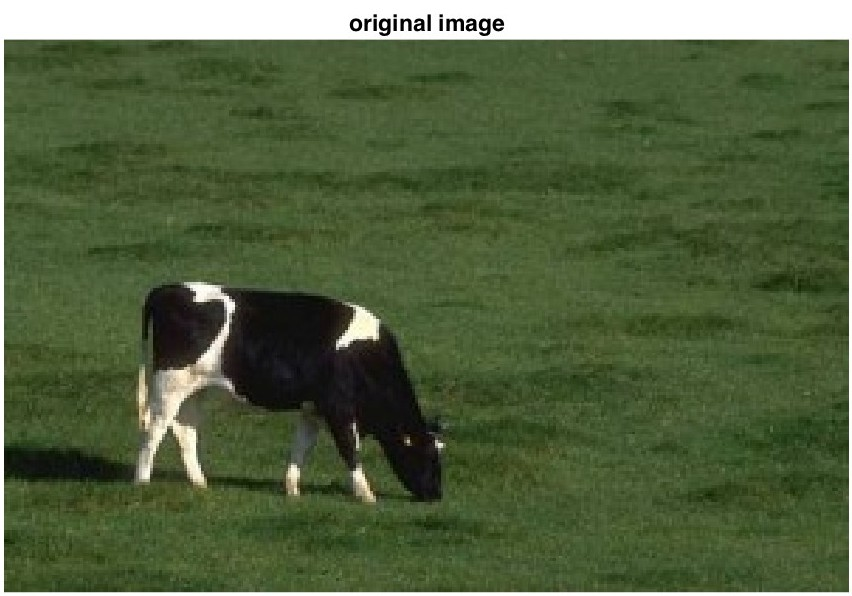
\includegraphics[width=1\linewidth]{images/original}
    \end{subfigure}%
    \begin{subfigure}[b]{.5\textwidth}
        \centering
        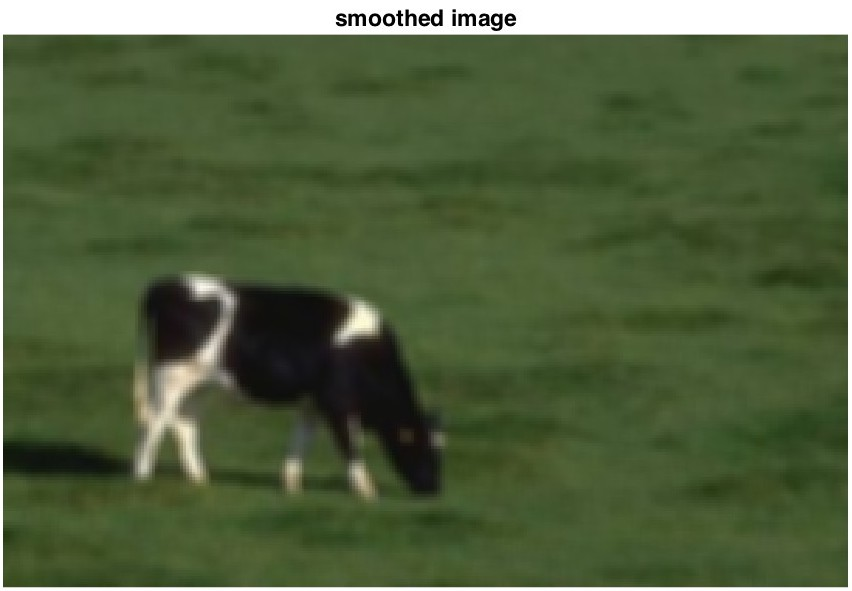
\includegraphics[width=1\linewidth]{images/smoothed}
    \end{subfigure}
    \caption{Effect of the smoothing filter.}
    \label{fig:smoothing}
\end{figure}

The second step of the preprocessing is to change the color representation.
The original image use the RGB space, while the one used for the segmentation is the L*a*b color space.
This color space is used in segmentation as it makes easier to differ from different colors as is designed to approximate human vision.

\begin{figure}[h]
    \centering
    \begin{subfigure}[b]{.5\textwidth}
        \centering
        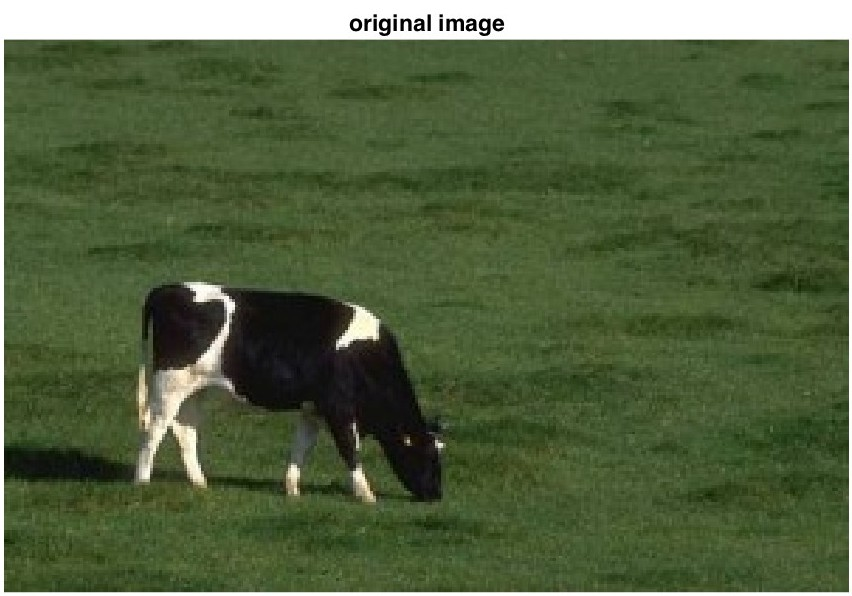
\includegraphics[width=1\linewidth]{images/original}
    \end{subfigure}%
    \begin{subfigure}[b]{.5\textwidth}
        \centering
        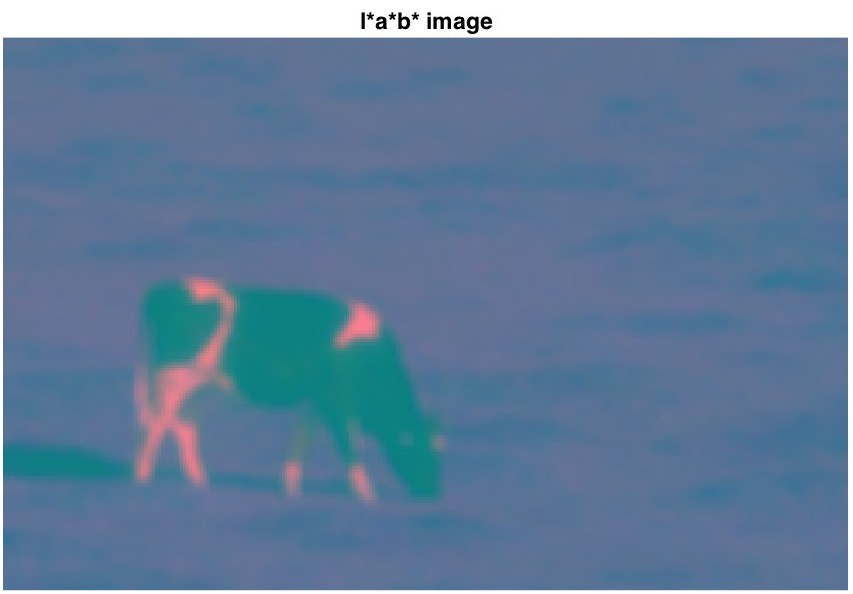
\includegraphics[width=1\linewidth]{images/img_Lab}
    \end{subfigure}
    \caption{Effect of the color space transformation.}
    \label{fig:color_transform}
\end{figure}

\section*{Mean-Shift Segmentation}




\section*{EM Segmentation}

The second task is to perform the segmentation using the EM algorithm.
This algorithm models a fixed number of $K$ segments as Gaussian distributed in the color space forming a Gaussian Mixture Model with each segment weighted.
The algorithm to compute the segmentation, consists in two steps.
The first is to estimate the probability of each pixel belonging to each of the segments defined by its distribution.
The second consist in updating the parameters of the Gaussian distributions of each segment in order to maximize the total log likelihood.

The \textbf{E step} of the algorithm computer the responsibilities of each pixel to each segment.
Then, the \textbf{M step} consist in the update of the parameters given the previous expectation in order to maximize the total log likelihood.

To run the EM algorithm, it is required first, to initialize the parameters $\alpha_k$, $\mu_k$ and $\Sigma_k$. This values have been initialized taking into account the distribution of all the pixels along all the color space.

Once the initialization is done, the EM algorithm iterate computing the estimation step and the maximization step until convergence.
The converges is defined when the total log likelihood at each step does not improve more than a tolerance respect the previous step.

\subsection*{Segmentation results}

Now I am going to give the results of the EM algorithm for different number of segments. The results will consist on the parameters $\Theta$ of the Gaussian Mixture Model, as well as the segmented image.

\subsubsection*{$K=3$}

\begin{equation}
    \alpha_k = \begin{bmatrix}
        0.8549 & 0.1065 & 0.0386
    \end{bmatrix}
\end{equation}

\begin{equation}
    \mu_k = \begin{bmatrix}
        0.3481  &  0.4470  &  0.5824 \\
        0.1652  &  0.4822  &  0.5356 \\
        0.5328  &  0.4886  &  0.5496
    \end{bmatrix}
\end{equation}

\begin{equation}
    \begin{split}
        \Sigma_1&= \begin{bmatrix}
            0.8596 &  0.0050 &  0.0062 \\
            0.0050 &  0.0127 & -0.0026 \\
            0.0062 & -0.0026 &  0.0234
        \end{bmatrix} \cdot 10^{-3},
        \Sigma_2 = \begin{bmatrix}
            0.0124 & -0.0021 &  0.0037 \\
            -0.0021 &  0.0005 & -0.0007 \\
            0.0037 & -0.0007 &  0.0012
        \end{bmatrix}, \\
        \Sigma_3&= \begin{bmatrix}
            0.0361 &  0.0012 &  0.0005 \\
            0.0012 &  0.0002 & -0.0001 \\
            0.0005 & -0.0001 &  0.0004
        \end{bmatrix}
    \end{split}
\end{equation}

\begin{figure}[h]
    \centering
    \begin{subfigure}[b]{.5\textwidth}
        \centering
        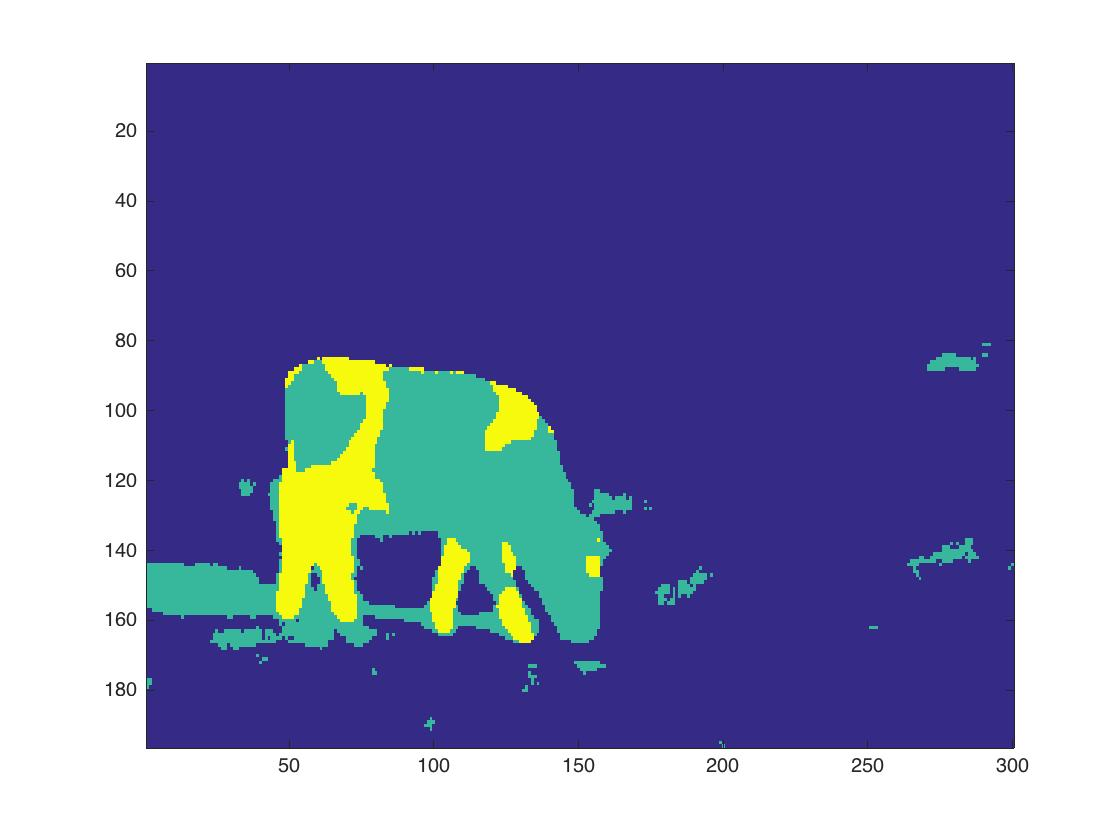
\includegraphics[width=1\linewidth]{images/seg_K_3}
    \end{subfigure}%
    \begin{subfigure}[b]{.5\textwidth}
        \centering
        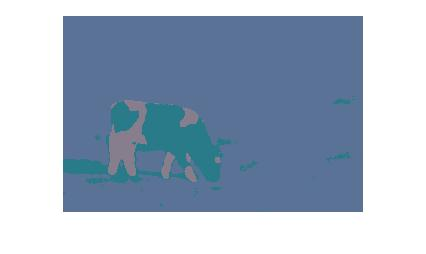
\includegraphics[width=1\linewidth]{images/seg_K_3_color}
    \end{subfigure}
    \caption{Segmentation using 3 segments.}
    \label{fig:seg_k3}
\end{figure}

\subsubsection*{$K=4$}

\begin{equation}
    \alpha_k = \begin{bmatrix}
     0.0780 & 0.3987 & 0.4777 & 0.0455
    \end{bmatrix}
\end{equation}

\begin{equation}
    \mu_k = \begin{bmatrix}
        0.3708 & 0.4822 & 0.5479 \\
        0.3622 & 0.4474 & 0.5798 \\
        0.3342 & 0.4468 & 0.5847 \\
        0.0609 & 0.5025 & 0.5028
    \end{bmatrix}
\end{equation}

\begin{equation}
    \begin{split}
        \Sigma_1&= \begin{bmatrix}
            0.0474 & 0.0012 & 0.0013 \\
            0.0012 & 0.0003 &-0.0002 \\
            0.0013 &-0.0002 & 0.0004
        \end{bmatrix},
        \Sigma_2= \begin{bmatrix}
            0.2681 &  0.0020 & -0.0007 \\
            0.0020 &  0.0060 & -0.0004 \\
            -0.0007 & -0.0004 &  0.0073
        \end{bmatrix} \cdot 10^{-3}, \\
        \Sigma_3&= \begin{bmatrix}
            0.0011 & -0.0000 &  0.0001 \\
            -0.0000 &  0.0000 & -0.0000 \\
            0.0001 & -0.0000 &  0.0000
        \end{bmatrix},
        \Sigma_4= \begin{bmatrix}
            0.3022 &  0.0499 &  0.0075 \\
            0.0499 &  0.0412 & -0.0147 \\
            0.0075 & -0.0147 &  0.0516
        \end{bmatrix} \cdot 10^{-3}
    \end{split}
\end{equation}

\begin{figure}[h]
    \centering
    \begin{subfigure}[b]{.5\textwidth}
        \centering
        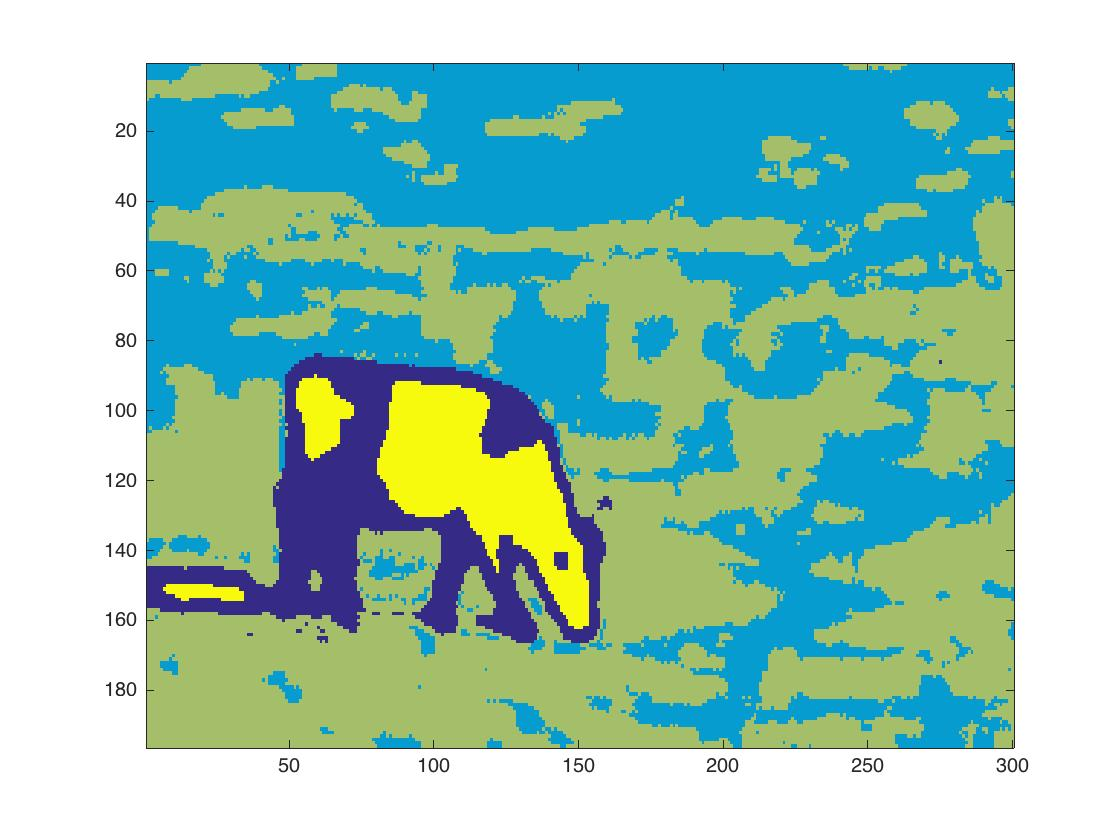
\includegraphics[width=1\linewidth]{images/seg_K_4}
    \end{subfigure}%
    \begin{subfigure}[b]{.5\textwidth}
        \centering
        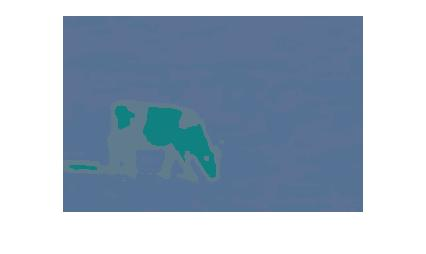
\includegraphics[width=1\linewidth]{images/seg_K_4_color}
    \end{subfigure}
    \caption{Segmentation using 4 segments.}
    \label{fig:seg_k4}
\end{figure}

\subsubsection*{$K=5$}

\begin{equation}
    \alpha_k = \begin{bmatrix}
        0.0443 & 0.0781 & 0.3401 & 0.2666 & 0.2708
    \end{bmatrix}
\end{equation}

\begin{equation}
    \mu_k = \begin{bmatrix}
        0.0599 & 0.5026 & 0.5024 \\
        0.3669 & 0.4828 & 0.5468 \\
        0.3635 & 0.4470 & 0.5795 \\
        0.3556 & 0.4477 & 0.5847 \\
        0.3175 & 0.4466 & 0.5841
    \end{bmatrix}
\end{equation}

\begin{equation}
    \begin{split}
        \Sigma_1&= \begin{bmatrix}
            0.2657 &  0.0492 & -0.0029 \\
            0.0492 &  0.0390 & -0.0134 \\
            -0.0029 & -0.0134 &  0.0474
        \end{bmatrix} \cdot 10^{-3},
        \Sigma_2= \begin{bmatrix}
            0.0486 &  0.0011 &  0.0015 \\
            0.0011 &  0.0003 & -0.0002 \\
            0.0015 & -0.0002 &  0.0004
        \end{bmatrix}, \\
        \Sigma_3&= \begin{bmatrix}
            0.2450 &  0.0085 & -0.0019 \\
            0.0085 &  0.0062 & -0.0008 \\
            -0.0019 & -0.0008 &  0.0065
        \end{bmatrix} \cdot 10^{-3},
        \Sigma_4= \begin{bmatrix}
            0.5934 & -0.0306 &  0.0627 \\
            -0.0306 &  0.0105 & -0.0078 \\
            0.0627 & -0.0078 &  0.0246
        \end{bmatrix} \cdot 10^{-3}, \\
        \Sigma_5&= \begin{bmatrix}
            0.8418 &  0.0056 &  0.0649 \\
            0.0056 &  0.0294 &  0.0010 \\
            0.0649 &  0.0010 &  0.0292
        \end{bmatrix} \cdot 10^{-3}
    \end{split}
\end{equation}

\begin{figure}[h]
    \centering
    \begin{subfigure}[b]{.5\textwidth}
        \centering
        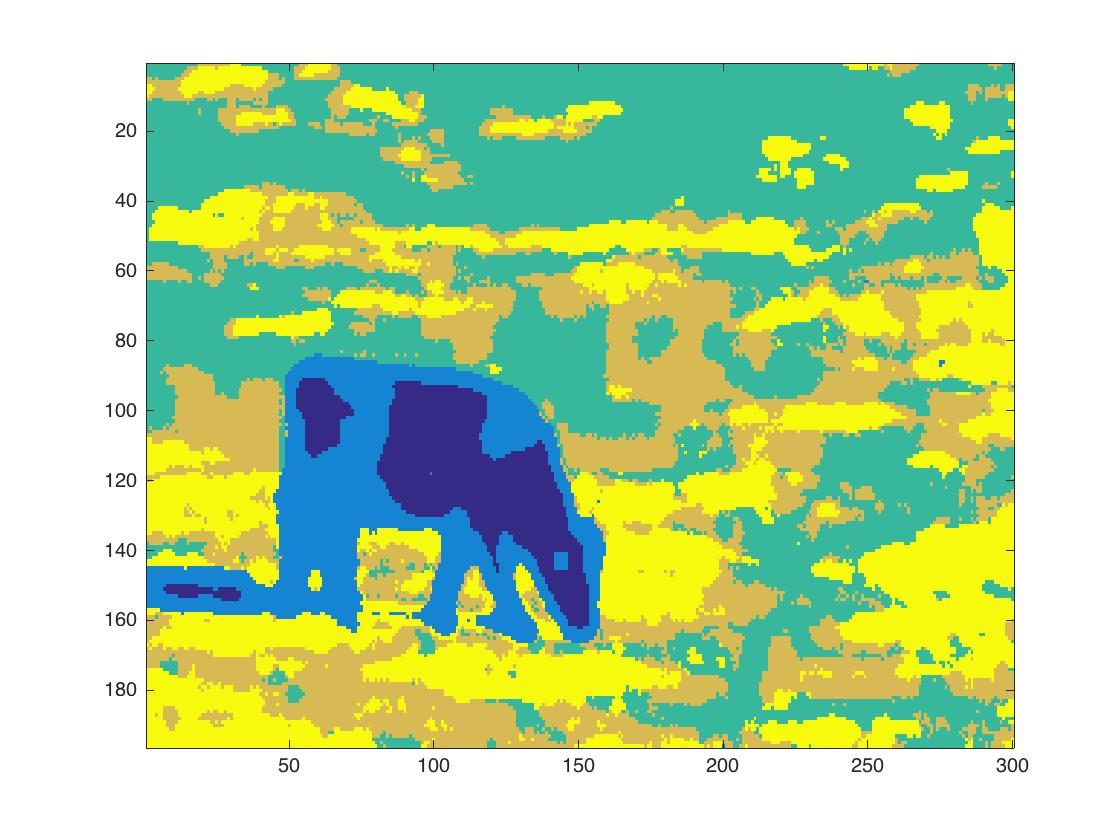
\includegraphics[width=1\linewidth]{images/seg_K_5}
    \end{subfigure}%
    \begin{subfigure}[b]{.5\textwidth}
        \centering
        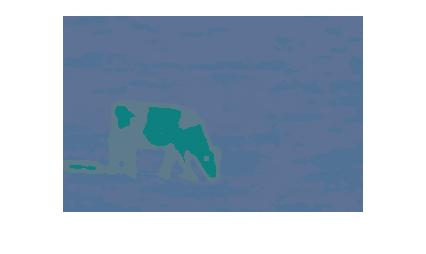
\includegraphics[width=1\linewidth]{images/seg_K_5_color}
    \end{subfigure}
    \caption{Segmentation using 5 segments.}
    \label{fig:seg_k5}
\end{figure}

\end{document}
